% !TEX TS-program = pdflatex
% !TEX encoding = UTF-8 Unicode

\documentclass[a4paper, titlepage=false, parskip=full-, 10pt]{scrartcl}

\usepackage[utf8]{inputenc}
\usepackage[T1]{fontenc}
\usepackage[english, ngerman]{babel}
\usepackage{babelbib}
\usepackage{hyperref}
\usepackage{listings}
\usepackage{framed}
\usepackage{color}
\usepackage{graphicx}
\usepackage[normalem]{ulem}
\usepackage{cancel}
\usepackage{amsmath}
\usepackage{amssymb}
\usepackage{amsthm}
\usepackage{algorithm}
\usepackage{algorithmic}
\usepackage{geometry}
\usepackage{subfigure}
\geometry{a4paper, top=20mm, left=35mm, right=25mm, bottom=40mm}

\newcounter{tasknbr}
\setcounter{tasknbr}{1}
\newenvironment{task}[1]{{\bf Aufgabe \arabic {tasknbr}\stepcounter{tasknbr}} (#1):\begin{enumerate}}{\end{enumerate}}
\newcommand{\subtask}[1]{\item[#1)]}

% Listings -----------------------------------------------------------------------------
\definecolor{red}{rgb}{.8,.1,.2}
\definecolor{blue}{rgb}{.2,.3,.7}
\definecolor{lightyellow}{rgb}{1.,1.,.97}
\definecolor{gray}{rgb}{.7,.7,.7}
\definecolor{darkgreen}{rgb}{0,.5,.1}
\definecolor{darkyellow}{rgb}{1.,.7,.3}
\lstloadlanguages{C++,[Objective]C,Java}
\lstset{
escapeinside={§§}{§§},
basicstyle=\ttfamily\footnotesize\mdseries,
columns=fullflexible, % typewriter font look better with fullflex
keywordstyle=\bfseries\color{blue},
% identifierstyle=\bfseries,
commentstyle=\color{darkgreen},      
stringstyle=\color{red},
numbers=left,
numberstyle=\ttfamily\scriptsize\color{gray},
% stepnumber=5,
% numberfirstline=true,
breaklines=true,
% prebreak=\\,
showstringspaces=false,
tabsize=4,
captionpos=b,
% framexrightmargin=-.2\textwidth,
float=htb,
frame=tb,
frameshape={RYR}{y}{y}{RYR},
rulecolor=\color{black},
xleftmargin=15pt,
xrightmargin=4pt,
aboveskip=\bigskipamount,
belowskip=\bigskipamount,
backgroundcolor=\color{lightyellow},
extendedchars=true,
belowcaptionskip=15pt}

%% Enter current values here: %%
\newcommand{\lecture}{Algorithmische Geometrie SS15}
\newcommand{\tutor}{}
\newcommand{\assignmentnbr}{5}
\newcommand{\students}{Julius Auer, Alexa Schlegel}
%%-------------------------------------%%

\begin{document}  
{\small \textsl{\lecture \hfill \tutor}}
\hrule
\begin{center}
\textbf{Übungsblatt \assignmentnbr}\\
[\bigskipamount]
{\small \students}
\end{center}
\hrule

\begin{task}{Suchen in ebenen Unterteilungen}
\item[]
Sei $G=(V,E,F)$ die ebene Unterteilung mit Knoten, Kanten und Facetten, wobei die Anzahl der Kanten und Facetten asymtotisch durch die Anzahl Knoten begrenzt ist, also $|E|,|F|\in O(n),n=|V|$.

Idee ist, die Ebene vertikal entlang der y-Koordinaten der Punkte und horizontal entlang der Geraden, welche die vertikalen Trennlinien schneiden, aufzuteilen. Hierzu werden in einem Array $A$ (auf dem später eine Binärsuche ausgeführt werden kann) Dupel $(z_i,X_i)$ gespeichert, wobei $z_i$ die y-Koordinate einer Trennlinie ist und $X_i=\{(e_1,f_1),...,(e_m,f_m)\}$ ein Array (für spätere Binärsuche) in dem alle Strecken gespeichert werden, die zwischen $z_i$ und $z_{i+1}$ entlang einer Kante $e\in E$ verlaufen. Es kann nur $O(n)$ solche Strecken geben und aufgrund der Planarität von $G$ werden sich auch diese Strecken nie schneiden. Dadurch teilen die Strecken die ''Spalte'' zwischen $z_i$ und $z_{i+1}$ in $O(n)$ disjunkte Teilräume, für welche die jeweils zugehörige Facette $f_j\in F$ bestimmt werden kann:

\begin{algorithm}
\caption{$INIT(V=\{ (x_1,y_1),...,(x_n,y_n)\},E,A=\{ (z_1,X_1),...,(z_n,X_n)\})$}
\begin{algorithmic}[1]
\STATE{sort $V$ by y-coordinate}\\
\FOR{$\text{ \bf each }y_i\in \{y_1,...,y_n\}$}
\STATE{$z_i:=y_i$}\\
\ENDFOR
\FOR{$\text{ \bf each }z_i\in\{z_1,...,z_n\}$}
\FOR{$\text{ \bf each }e\in E$}
\IF{$e \text{ intersects vertical line through }z_i$}
\STATE{$f:=\text{ find face directly below }e\text{ and between }z_i\text{ and }z_{i+1}$}\\
\STATE{$X_i\leftarrow (e,f)$}\\
\ENDIF
\ENDFOR
\STATE{sort $X_i$ by y-coordinate of left intersection}\\
\STATE{copy $X_i$ to array}\\
\ENDFOR
\end{algorithmic}
\end{algorithm}

Speicherkomplexität ist offensichtlich $O(n^2)$ für das Array.

Zeitkomplexität ist insgesamt $O(n^3)$, gegeben durch:
\begin{itemize}
\item $O(n\cdot\log n)$ für Sortieren mit geeignetem Algorithmus (1-4)
\item $n$ Ausführungen der äußeren Schleife (5)
\item $O(n)$ Ausführungen der inneren Schleife (6)
\item in den Schleifen:
\begin{itemize}
\item konstante Zeit für die Operationen (7, 9-11)
\item $O(n)$ für das Finden der passenden Facette (8) wenn naiv alle Facetten ausprobiert werden
\item $O(n\cdot\log n)$ für Sortieren mit geeignetem Algorithmus (12)
\item $O(n)$ zur Umwandlung einer Liste in ein Array (13)
\end{itemize}
\end{itemize}

Nach dieser Vorverarbeitung kann für einen gegebenen Punkt $p=(x,y)$ mittels Binärsuche auf $\{ z_1,...,z_n\}$ die passende ''Spalte'' $z_i$ gefunden werden, und mit einer zweiten Binärsuche auf $X_i=\{(e_1,f_1),...,(e_m,f_m)\}$ die passende Facette gefunden werden, indem on-the-fly geprüft wird ob $p$ ober- oder unterhalb einer Strecke $e_j$ liegt. Der Algorithmus ist trivial und die Zeitkomplexität offensichtlich $O(\log n)$.
\end{task}

\begin{task}{$L_1$-Voronoi-Diagramme}
\item[]
In $L_1$-Metrik beschreiben die Punkte mit Abstand $d$ von einem Punkt ein Quadrat mit Seitenlänge $2\cdot d$ (Abb. \ref{fig:l1_1}).
\begin{figure}[h]
\begin{center}
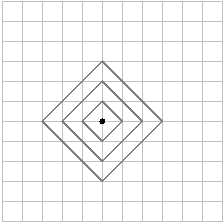
\includegraphics[width=3cm]{capture0}
\end{center}
\caption{Punkte mit Abständen 1,2,3 von einem Punkt liegen auf den Ränder dieser Quadrate}
\label{fig:l1_1}
\end{figure}

Eine zwei Voronoi-Regionen trennende Kante hat nun stets eine von drei möglichen Formen, welche vom Verhältnis zwischen der X-Differenz und der Y-Differenz der Punkte bestimmt wird. Dominiert die X-Differenz, wird die Kante senkrecht ''aussehen''. Dominiert die Y-Differenz, wird die Kante waagerecht ''aussehen''.

Es sind im Folgenden die drei Fälle abgebildet, dass bei zwei Punkten die Y-Differenz (Abb. \ref{fig:l1_2}), die X-Differenz (Abb. \ref{fig:l1_3}) oder keine der beiden (Abb. \ref{fig:l1_4}) dominiert.

Jede Abbildung zeigt die drei untergeordneten Fälle, bei denen der in der dominanten Dimension größere Punkt in der rezesiven Dimension kleiner/gleich/größer dem anderen Punkt ist. Andere Fälle als die gezeigten sieben kann es nicht geben.

\begin{figure}[h]
\begin{center}
\subfigure{
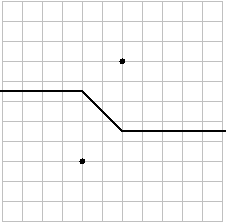
\includegraphics[width=3cm]{capture1}
}
\subfigure{
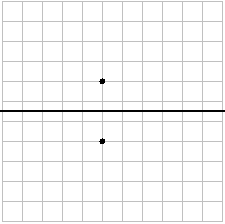
\includegraphics[width=3cm]{capture2}
}
\subfigure{
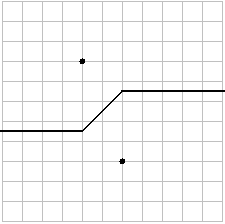
\includegraphics[width=3cm]{capture3}
}
\end{center}
\caption{Fall 1: $\left|\frac{x_1-x_2}{y_1-y_2}\right| <1$}
\label{fig:l1_2}
\end{figure}

\begin{figure}[h]
\begin{center}
\subfigure{
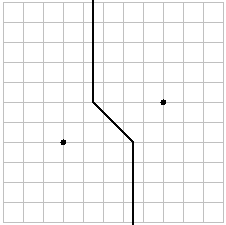
\includegraphics[width=3cm]{capture4}
}
\subfigure{
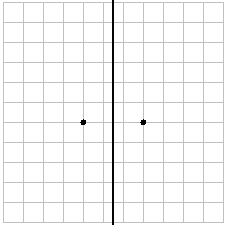
\includegraphics[width=3cm]{capture5}
}
\subfigure{
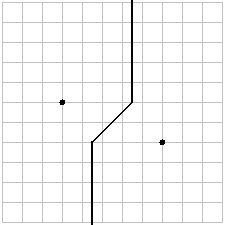
\includegraphics[width=3cm]{capture6}
}
\end{center}
\caption{Fall 2: $\left|\frac{x_1-x_2}{y_1-y_2}\right| >1$}
\label{fig:l1_3}
\end{figure}

\begin{figure}[h]
\begin{center}
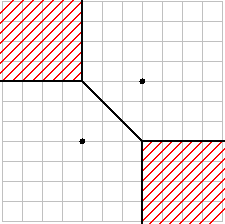
\includegraphics[width=3cm]{capture7}
\end{center}
\caption{Fall 3: $\left|\frac{x_1-x_2}{y_1-y_2}\right| =1$}
\label{fig:l1_4}
\end{figure}

Auffälig ist hier der letzte, entartete Fall, bei dem eine Menge von Punkten (rot) zu beiden Punkten equidistant ist und keine Kante sondern eine Fläche beschreibt. Wie dieser Fall im Kontext von Voronoi-Diagrammen behandelt werden sollte ist nicht aus deren Definition abzuleiten. In der Praxis sollte dieser Fall jedoch ohnehin nur relevant sein, wenn mit Ganzzahligen Koordinaten gerechnet wird.
\end{task}

\newpage
\begin{task}{Suche in ebenen Unterteilungen - Verallgemeinerung}
\item[]
Die Lokalisierungsdatenstruktur (LDS) wurde in der Vorlesung als gerichteter azyklischer Graph (DAG) beschrieben und funktioniert für ebene Unterteilungen, wo jede Facette ein Dreieck ist, auch die Außenfacette.

Wir werden nun im ersten Schritt aus der beliebigen Unterteilung der Ebene eine Triangulierung erzeugen - mit einem Dreieck als Außenfacette. Im zweiten Schritt wenden wir darauf den in der Vorlsung vorgestellten Algorithmus zur Konstruktion der LDS an.

\begin{enumerate}
\item Um die vorhandene Unterteilung $U$ ein großes Dreieck $D$ legen, sodass alle Kanten im Inneren des Dreicks liegen.
\item Schnittpunkte von $D$ mit Strahlen (Verlängerungen der Kanten) der Unterteilung $U$ als Knoten in $U$aufnehmen.
\item Eckpunkte des Dreiecks auch in $U$ aufnehmen.
\item Inneres von $U$ Triangulieren $\rightarrow G$.
\item Algorithmus zur Konstruktion der LDS($G$) anwenden.
\end{enumerate}

Folgendes wurde in der Vorlesung definiert:

\begin{itemize}
\item eingebetteter Graph $G$ entspricht $S_1$
\item $S_h$ ist das äußere, umschließende Dreieck
\item $h=O(\log n)$
\item $I$ ist die unabhängige Knotenmenge
\end{itemize}

\begin{algorithm}
\caption{Algorithmus zur Konstruktion der LDS($G$)}
\begin{algorithmic}[1]
\STATE Sei $S_1=G$
\STATE Für jedes $\triangle$ in $G$ erzeuge einen Knoten in LDS($G$)
\STATE i = 1
\WHILE {$|S_i|>3$}
    \STATE {Berechne von $I$}
    \STATE {Entferne $I$ aus $S_i$}
    \STATE {Trianguliere $S_i \setminus I \rightarrow S_i+1$}
    \STATE {für jedes neue $\triangle$ $t$ in $S_i+1$ erzeuge einen Knoten K($t$)in LDS($G$) und füge eine Kante von K($t$) zu allen Knoten von Dreiecken von $S_i$ die von  $t$ geschnitten werden}
    \STATE {i++}
\ENDWHILE
\end{algorithmic}
\end{algorithm}

\begin{algorithm}
\caption{Lokalisiere ($q$, LDS($G$))}
\begin{algorithmic}[1]
\IF {$q \not \in S_h$}
		\RETURN {$q$ liegt in Außenfacette}
\ENDIF
\STATE {$v$=Wurzel(LDS($G$))}
\WHILE {$v$ hat Nachfolger}
		\FORALL {Nachfolger $u$ von $v$}
    		\IF {$q$ ist in Dreieck von $u$}
    				\STATE {$v=u$}
    		\ENDIF
		\ENDFOR
\ENDWHILE
\RETURN {$q$ liegt im Dreieck von $v$}
\end{algorithmic}
\end{algorithm}

\begin{description}
\item[Vorverarbeitungszeit]
(a) dauert $O(n)$, um das min-$x$, max-$x$ zu finden. (b) benötigt ebenfalls $O(n)$ wenn naiv alle Kanten betrachtet werden.\\
$\rightarrow O(n)$
\item[Speicherbedarf]
Im schlimmsten Fall können $O(n)$ zusätzliche Knoten und genauso viele neue Kanten entstehen, die zusätzlichen Speicher benötigen.\\
$\rightarrow O(n)$
\item[Anfragezeit]
unverändert.\\
$\rightarrow O(\log n)$
\end{description}
\end{task}
\end{document}